In this section, we provide examples illustrating the typical 
optimal solution structures of \opglr and \opgmc computed by 
our DP algorithms. Using an application scenario, solutions to 
\opglr and \opgmc are also compared. Then, computational 
results from extensive numerical evaluations are presented, 
confirming the effectiveness of these algorithms. The 
implementation is done using the Python and all 
computations are performed on an Intel(R) Core(TM) i7-7700 CPU@3.6GHz 
with 16GiB RAM. 

\subsection{Basic Optimal Solution Structure}
~\ref{fig:opgext-opglrm} shows the typical outcome of solving an \opglr 
instance with two perimeters ($m = 2$) for two types of robots with 
$n_1 = 3, a_1 = 5$, and $n_2 = 5, a_2 = 8$. 
%That is, the second type of robots is more capable than the first type. 
In the figure, the red segments are parts of the two perimeters that 
must be guarded. The three orange (resp., five green) segments across 
the two perimeters indicate the desired coverage regions of the three 
(resp., five) type $1$ (resp., type $2$) robots. These coverage regions 
correspond to the optimal solution returned by the DP algorithm. As 
may be observed, the optimal solution is somewhat complex with robots 
of both types on each of the two perimeters; a gap on the second boundary 
also gets covered. The coverage lengths for a robot type are generally 
different; this is due to adjustments that shrink some robots' coverage. 
For example, the first perimeter has a very short orange cover because 
the corresponding perimeter segment is short and gaps around it need 
not be covered (The adjustment procedure is also shown in the video). 
\begin{figure}[!ht]
    \centering
    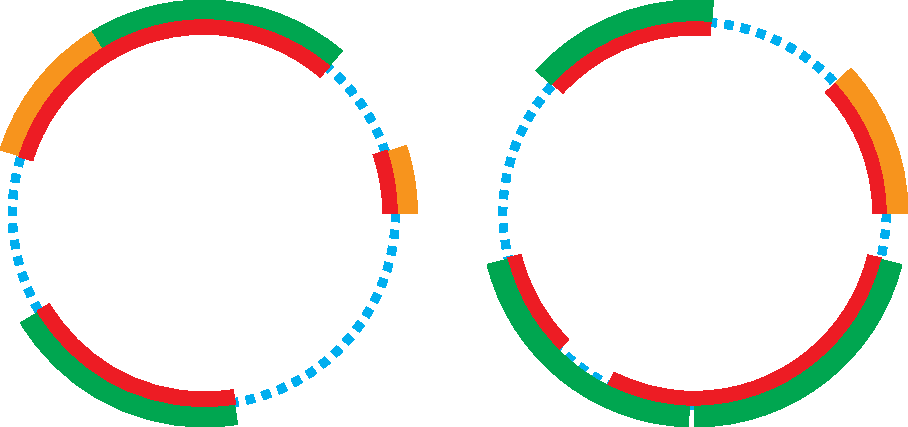
\includegraphics[scale = 0.6]{chapters/opg-ext/figures/mopglr_shrink-new-eps-converted-to.pdf}
    \caption[An \opglr problem and an associated optimal solution]
    {An \opglr problem and an associated optimal solution. The 
		problem has two perimeters and $t = 2$ with $n_1$=3, $n_2$=5, 
		$a_1$=5, $a_2$=8. The boundaries are shown as circles for ease of 
		illustration.
		%, which does not affect the computation or the solution.
		}
		\label{fig:opgext-opglrm}
\end{figure}

Shifting our attention to \opgmc, ~\ref{fig:opgext-opgmc} illustrates the 
structure of an optimal solution to a problem with three types of robots 
with capacities and costs being $\ell_1=11, c_1=2$, $\ell_t=30, 
c_2=4$, and $\ell_3=55, c_3=7$, respectively. In this case, the majority 
of the deployed robots are of type $2$ with $\ell_2=30, c_2=4$. Only one 
type $1$ and one type $3$ robots are used. The four perimeter segments are 
covered by three robot groups. 
%
%To clearly illustrate the solution structure, the combined coverage of each 
%robot group runs beyond the counterclockwise direction of the corresponding 
%segments being covered (e.g., the counterclockwise end of the orange segment 
%is inside a gap). 
%
The only type $3$ robot guards (the purple segment) across two different 
perimeter segments. Coverage length adjustment is also performed to avoid 
the unnecessary coverage of some gaps. 

\begin{figure}[!ht]
    \centering
    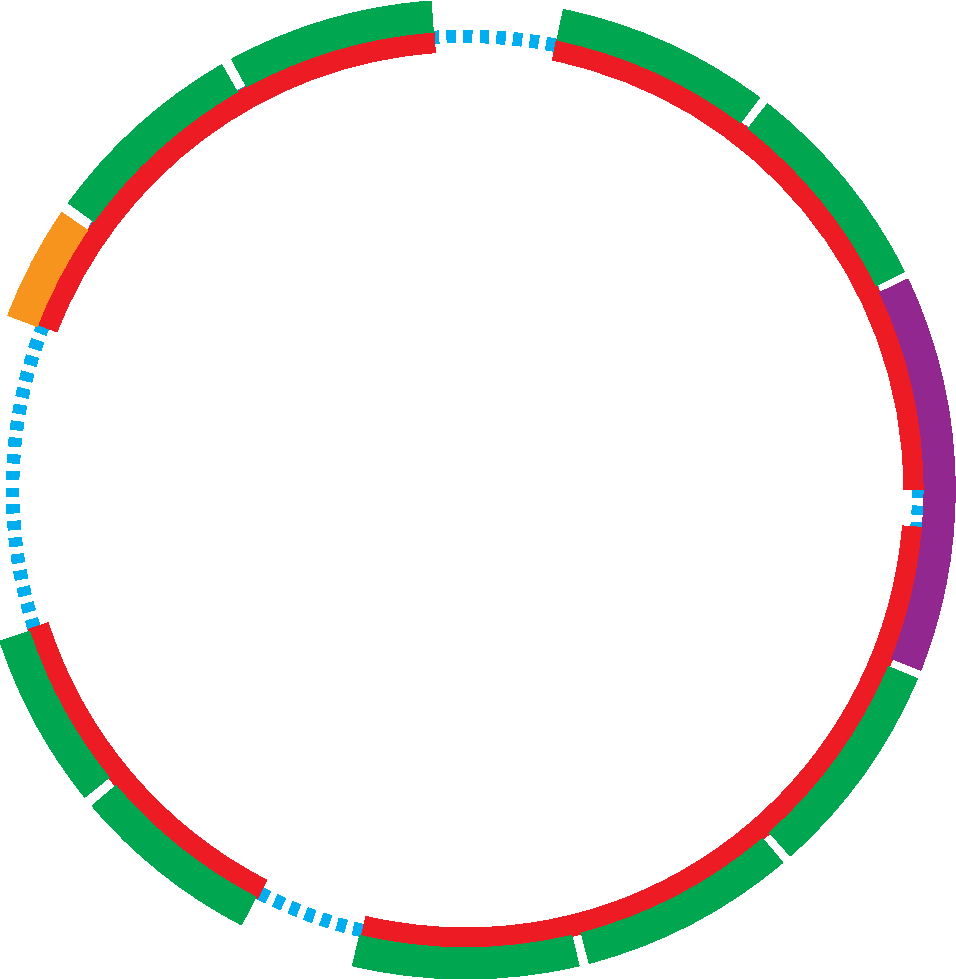
\includegraphics[scale = 0.4]{chapters/opg-ext/figures/opgmc-new-t-eps-converted-to.pdf}
    \caption[An \opgmc problem and an associated optimal solution]
    {An \opgmc problem and an associated optimal solution. The 
		problem has four (red) perimeter segments and three types of robots
		with $\ell_1=11, c_1=2$ (orange), $\ell_t=30, c_2=4$ (green), 
		and $\ell_3=55, c_3=7$ (purple), respectively.}
		\label{fig:opgext-opgmc}
\end{figure}

\subsection{A Robotic Guarding and Patrolling Application}
In this subsection, as a potential application, the DP algorithms for 
\opglr and \opgmc are employed to solve the problem of securing the 
perimeter of the Edinburgh castle, an example used in 
\cite{fenghangaoyu2019efficient}. As shown in ~\ref{fig:opgext-castle} (minus 
the orange and green segments showing the solutions), the central 
region of the Edinburgh castle has tall buildings on its boundary 
(the blocks in brick red); these parts of the boundary are the gaps 
that do not need guarding. In the figure, the top sub-figure shows 
the optimal solution for an \opglr instance and an \opgmc instance with 
a total of $11$ robots. The bottom sub-figure is a slightly updated 
\opgmc instance with slightly higher $c_2$. 
\begin{figure}[!ht]
    \centering
    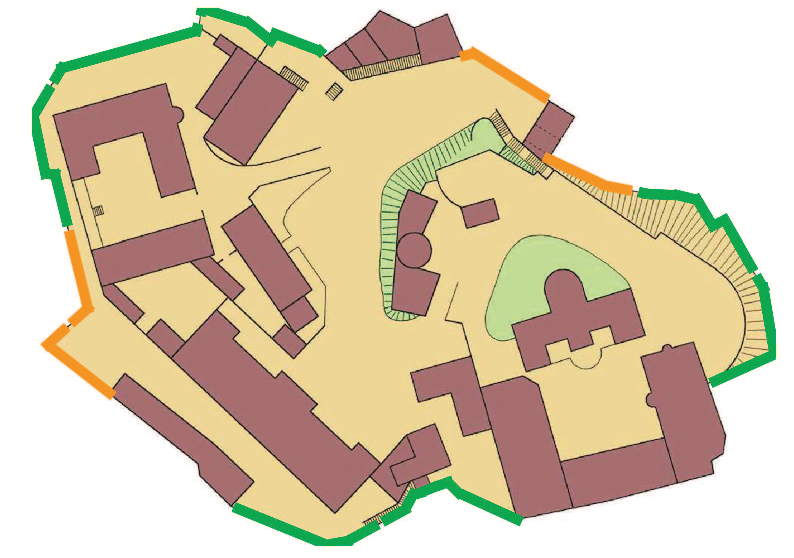
\includegraphics[scale = 0.5]{chapters/opg-ext/figures/opglr-castle-thin-eps-converted-to.pdf}
    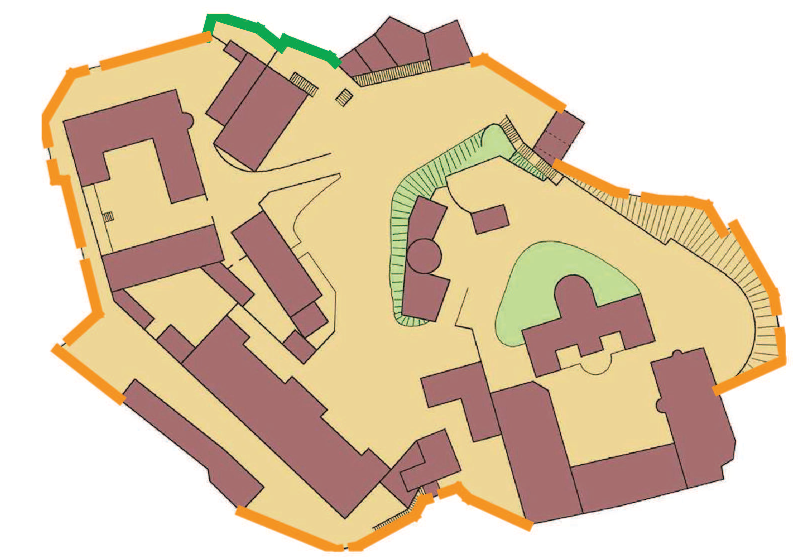
\includegraphics[scale = 0.5]{chapters/opg-ext/figures/opgmc-castle-thin-eps-converted-to.pdf}
    \caption[\opglr and \opgmc instances solutions]{[left] \opglr solution with $n_1 = 4, n_2 = 7, 
		c_1:c_2 = 2:3$ and \opgmc solution with $\ell_1 = 150, 
		c_1 = 100, \ell_2 = 225, c_2 = 145$, and total boundary $3058$. Cost 
		of \opgmc solution is $1415$.
		[right] \opgmc solution with $\ell_1 = 150, c_1 = 100, \ell_2 = 
		225, c_2 = 155$. Cost of solution ($13$ type $1$, $1$ type $2$) is 
		$1455$.
		%
		In both solutions, covers by type $1$ (resp., 
		type $2$) robots are shown in orange (resp., green).
		%, which does not affect the computation or the solution.
		}
		\label{fig:opgext-castle}
\end{figure}

It can be observed that the results, while having non-trivial structures, 
make intuitive sense. For the top sub-figure, solutions to both \opglr 
and \opgmc (because robot with larger capacity is slightly lower in 
relative cost) use mainly higher capacity robots to cover longer perimeter 
segments and use the lower capacity robots mostly fillers. The solution 
covers a small gap at the bottom. For the bottom sub-figure, while only 
small changes are made to the cost, because the longer segment is more 
expensive to use now, the first type of robot is used mainly. 

\subsection{Computational Performance}
With Section~\ref{sec:opgext-algorithm} fully establishing the correctness and 
asymptotic complexity of the pseudo-polynomial time algorithms, here, the 
running time of these algorithms are experimentally evaluated. In doing 
so, the main goal is demonstrating that, despite the hardness of \opglr 
and \opgmc, the proposed algorithms could solve the target problems under 
reasonably broad settings in a scalable way. For results presented in 
this subsection, each data point is an average over 10 randomly generated 
instances. 

The first two numerical evaluations (\ref{tab:opgext-opglr} and 
~\ref{tab:opgext-mopglr}) focus on the running times of the pseudo-polynomial 
time algorithms for \opglr over single and multiple perimeters, 
respectively. In these two tables, $t$ and $q$ are the number of types 
and the number of segments, respectively. For each type $\tau$, a 
capacity ($a_{\tau}$) is randomly sampled as an integer between $1$ and 
$100$, inclusive. The number of robots available for each type ($n_{\tau}$) 
is sampled uniformly between $5$ and $15$, inclusive. For the multiple 
perimeters case, the parameter $m$ represents the number of perimeters for 
a given instance.

For the single perimeter case (\ref{tab:opgext-opglr}), the results show 
that the pseudo-polynomial time algorithm is effective for up to five 
types of robots, for dozens of robots. We expect a more efficient 
(e.g., C++ based) implementation should be able to effectively handle 
up to five types of robots with the total number of robots being around 
a hundred, on a typical PC. This is likely sufficient for many practical 
applications which have limited types and numbers of robots. Since the 
algorithm has exponential dependency on $t$, it becomes less efficient 
for larger $t$ as expected.  

\begin{table}[htbp]
	\centering
	\begin{tabularx}{\columnwidth}{|c|X|X|X|X|X|X|}
		\hline
%		\renewcommand{\arraystretch}{0.99}
		\diagbox{$t$}{$q$}&  \quad 5 &   \quad 10 &\quad 20& \quad 30 & \quad 40&\quad 50 \\
		\hline
		\renewcommand{\arraystretch}{1.05}
		2&0.022 &0.044 &0.131 &0.208 &0.326 &0.516 \\\hline
        3&0.281 &0.714 &1.670 &2.577 &4.107 &4.708 \\\hline
        4&5.504 &16.07 &41.68 &71.55 &109.9 &138.9 \\\hline
        5&29.53 &75.60 &243.6 &443.4 &528.0 &725.0 \\\hline
	\end{tabularx}
	\caption{Running time in seconds used by the DP algorithm for \opglr over 
	a single perimeter.
	}
	\label{tab:opgext-opglr}
\vspace*{-1mm}
\end{table}

\ref{tab:opgext-mopglr} illustrates the running time of the DP algorithm for 
\opglr over multiple perimeters. As can be readily observed, the impact of 
the number of perimeters $m$ on the running time is relatively small; the 
number of robot types is still the determining factor for running time. In 
this case, our proposed solution is effective for $t$ up to $4$ and starts to 
slow down a robot types become larger than $4$. 
\begin{table}[htbp]
	\centering
	\renewcommand{\arraystretch}{1.05}
    \begin{tabularx}{\columnwidth}{|c|X|X|X|X|X|X|}
        \hline
        {\multirow{2}{*}{\diagbox{$m$}{$q$}} }&\multicolumn{2}{c|}{10}&\multicolumn{2}{c|}{20}&\multicolumn{2}{c|}{30} \\
        \cline{2-7}
         &\,\,\,$t$=3 & $\,\,\,t$=4& $\,\,\,t$=3 & $\,\,\,t$=4& \,\,\,$t$=3  & \,\,\,$t$=4\\
        \hline
        2&3.148 &133.2 &7.077 &198.4 &10.33 &260.0 \\\hline
        3&4.828 &194.1 &10.125 &290.6 &15.52 &376.7 \\\hline
        4&6.131 &256.8 &12.485 &381.3 &19.75 &514.3 \\\hline
        5&7.622 &321.7 &15.355 &476.2 &24.31 &605.8 \\\hline
    \end{tabularx}
    \caption{Running time in seconds used by the DP algorithm for \opglr over multiple perimeters.}
    \label{tab:opgext-mopglr}
\vspace*{-1mm}
\end{table}

Table~\ref{tab:opgext-opgmc} provides performance evaluation of \opgmcdp. Since 
there is no difference between single and multiple perimeters for \opgmc,
only problems with single perimeters are attempted. Here, for each robot 
type, the cost is an integer randomly sampled between $1$ and $20$, and 
the capacity is computed as five times the cost plus a random integer 
between $1$ and $20$. In the table, $L = \partial R$, the total length 
of the entire boundary. 
%
Given \opgmc's lower computational complexity, the DP algorithm, 
\opgmcdp, can effectively deal with over a few hundred types of robots 
with ease. 
\begin{table}[!ht]
	\centering
	\renewcommand{\arraystretch}{1.04}
    \begin{tabularx}{\columnwidth}{|c|X|X|X|X|X|X|}
        \hline
        \multirow{2}{*}{\diagbox{$t$}{$L$}} & 
        \multicolumn{2}{c|}{$10^2$}&\multicolumn{2}{c|}{$10^4$} &\multicolumn{2}{c|}{$10^6$} \\
        \cline{2-7}
        &$q$=20&$q$=50&$q$=20&$q$=50&$q$=20&$q$=50\\
        \hline
        3&0.006 &0.064 &0.041 &0.098 &3.040 &3.144 \\\hline
        10&0.005 &0.066 &0.094 &0.155 &9.423 &9.409 \\\hline
        30&0.009 &0.070 &0.261 &0.320 &26.10 &28.59 \\\hline
        100&0.014 &0.077 &0.910 &0.969 &91.28 &93.20 \\\hline
        300&0.030 &0.091 &2.652 &2.938 &275.6 &270.7 \\\hline
    \end{tabularx}
    \caption{Running time in seconds used by \opgmcdp algorithm.}
    \label{tab:opgext-opgmc}
\end{table}
\vspace*{-1mm}
\begin{comment}
    Application 1: for a single large region with a perimeter that may be viewed as straight line segments locally, we want to deploy multiple types of robots with different sensing radius. The goal is to ensure full coverage of the perimeter. Both problems formulations can be used. 

This also raises a related problem: what if we want to use discs to cover perimeter when a segment cannot be treated as straight lines? Can we also do tiling somehow? 

Another question: if we just use the same number of robots as used in an optimal cover to do a random feasible tiling, what would be the worst sub-optimality ratio? 

Application 2:  a multi-region application?
\end{comment}